\documentclass{beamer}
\setbeamertemplate{footline}[frame number]

\usepackage[utf8x]{inputenc}
\usepackage[brazil,british]{babel}
\usetheme{default} 
\usecolortheme{beaver}
\newtranslation[to=brazil]{Theorem}{Teorema}
\newtranslation[to=brazil]{Definition}{Definição}
\newtranslation[to=brazil]{Example}{Exemplo}
\newtranslation[to=brazil]{Problem}{Exercício}
\newtranslation[to=brazil]{Solution}{Resolução}
\logo{
\includegraphics[width=1cm]{../img/logo-ppgsc-icon-text.png}}

\usepackage{graphicx}
\usepackage{clrscode3e}
\usepackage{hyperref}

\usepackage{pgf}
\usepackage{tikz}
\newcommand{\assert}[1]{\textcolor{blue}{#1}}



\usepackage{pgf}
\usepackage{tikz}

\title{Aula 04: Análise de algoritmos --- notações asintóticas e classes de complexidade}
\author{David Déharbe \\
  Programa de Pós-graduação em Sistemas e Computação \\
  Universidade Federal do Rio Grande do Norte \\
  Centro de Ciências Exatas e da Terra \\
  Departamento de Informática e Matemática Aplicada}
\date{}

\begin{document}
\selectlanguage{brazil}

\begin{frame}
  \titlepage
\end{frame}

\begin{frame}

  \frametitle{Bibliografia usada}

  \begin{center}
    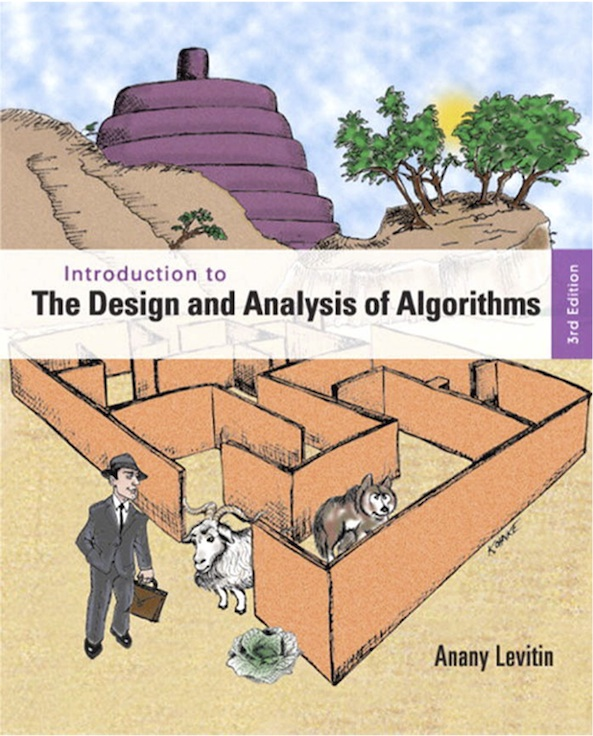
\includegraphics[height=.8\textheight]{img/capa-levitin.jpg}
  \end{center}
  (seção 2.2)
\end{frame}

\begin{frame}

  \frametitle{Estrutura da apresentação}

  \begin{enumerate}
  \item arcabouço teórico;
  \item melhor caso, pior caso, caso médio;
  \item \alert{notações asintóticas; $O$, $\Omega$, $\Theta$};
  \item análise de algoritmos não recursivos;
  \item análise de algoritmos recursivos.
  \end{enumerate}
\end{frame}

\begin{frame}
  \frametitle{Plano da aula}
  \tableofcontents
\end{frame}

\section{Introdução informal}

\begin{frame}
  \frametitle{Introdução}

  \begin{block}{Notações}
    Para um determinado algoritmo, $t(n)$ denota o tempo de execução (geralmente o contador de operações básicas $C(n)$).

    $g(n)$ denota uma função, que é comparada com $t(n)$.

    O objeto da comparação é o crescimento asintótico das funções.

  \end{block}
\pause
\begin{itemize}
\item 
\only<2>{
$O(g(n))$ é o conjunto das funções com um crescimento asintótico 
  \alert{menor ou igual} ao de $g(n)$.

    $n \in O(n^2), \quad 100n+5 \in O(n^2), \quad \frac{1}{2}n(n-1) \in O(n^2).$

    $n^3 \not\in O(n^2), \quad 0,000001n^3 \not\in O(n^2), \quad n^4 + n + 1 \not\in O(n^2).$
}
\pause
\only<3>{
$\Omega(g(n))$ é o conjunto das funções com um crescimento asintótico
  \alert{maior ou igual} ao de $g(n)$.

  $n^3 \in \Omega(n^2), \quad \frac{1}{2}n(n-1) \in \Omega(n^2), \quad 100n+5 \not\in \Omega(n^2).$
}
\pause
\only<4>{
$\Theta(g(n))$ é o conjunto das funções com um crescimento
  asintótico \alert{igual} a (um múltiplo positivo constante) de
  $g(n)$: $\Theta(n) = O(n) \cap \Omega(n)$.

  $an^2 + bn + c \in \Theta (n^2) \mbox{ se } a > 0, \quad n^2 + \log n \in \Theta(n^2).$
}
\end{itemize}

\end{frame}

\begin{frame}
\frametitle{Exercício}
\begin{enumerate}
\item Entre $O$, $\Omega$ e $\Theta$, qual a notação mais apropriada para discutir a complexidade:
\begin{itemize}
\item no pior caso;
\item no melhor caso;
\item em média?
\end{itemize}
\item Aplique as definições informais para determinar se as seguintes asserções
  são verdadeiras ou falsas:
\begin{itemize}
  \item $n(n+1)/2 \in O(n^3)$;
  \item $n(n+1)/2 \in O(n^2)$;
  \item $n(n+1)/2 \in \Theta(n^3)$;
  \item $n(n+1)/2 \in \Omega(n)$.
\end{itemize}
\end{enumerate}
\end{frame}

\section{Notação \texorpdfstring{$O$}{Big Oh}}

\begin{frame}
\frametitle{Notação $O$}
\begin{definition}
Uma função $t(n)$ é classificada como $O(g(n))$, e escreve-se $t(n) \in O(g(n))$ se $t(n)$ tem como limite superior um múltiplo constante de $g(n)$, ou seja
$$
\exists n_0, k \cdot \forall n \cdot n \ge n_0 \Rightarrow t(n) \le k \times g(n).
$$
\end{definition}
\end{frame}

\begin{frame}
  \frametitle{Ilustração: $t(n) \in O(g(n))$}
  \begin{center}
    \begin{tikzpicture}
  \draw[->](0, 0) -- (5, 0)             node[below] {$n$};
  \draw[->](0, 0) -- (0, 5);
  \draw[densely dotted](1, 5) -- (1, 0) node[below] {$n_0$};
  \node[rotate=90] at (0.5, 2.5) {n\~{a}o importa};
  \draw[color=red] (1, 1.5) .. controls (2, 2) and (3, 2.8) .. (5, 5) node[above]{$k g(n)$};
  \draw (1, 1.3) .. controls (2, 1.8) and (3, 2.6) .. (5, 4.5) node[above,right]{$t(n)$};
\end{tikzpicture}
  \end{center}
$$
t(n) \in O(g(n)) \equiv \exists n_0, k \cdot \forall n \cdot n \ge n_0 \Rightarrow t(n) \le k \times g(n).
$$
\end{frame}

\begin{frame}
\frametitle{Exemplo}

\begin{definition}
$t(n) \in O(g(n))$ sse $\exists n_0, k \cdot \forall n \cdot n \ge n_0 \Rightarrow t(n) \le k \times g(n)$.
\end{definition}

\begin{example}
Mostrar que $100n + 5 \in O(n^2)$.
\end{example}

\only<1>{\begin{proof}
  \begin{itemize}
    \item Se $n \ge 5$, então $100n + 5 \le 100 n + n = 101n$.
    \item Se $n \ge 1$, então $101n \le 101 n^2$.
    \item Temos $\forall n \cdot n \ge 5 \Rightarrow \underbrace{100n +
        5}_{t(n)} \le \underbrace{101 n^2}_{g(n)}$.
    \end{itemize}

    Ou seja, podemos usar os valores $101$ e $5$ como valores de $k$ e $n_0$ da
    definição.
\end{proof}
}
\only<2>{\begin{proof}
  \begin{itemize}
    \item Se $n \ge 1$, então $100n + 5 \le 100 n + 5n = 105n$.
    \item Se $n \ge 1$, então $105 n \le 105 n^2$.
    \item Temos $\forall n \cdot n \ge 1 \Rightarrow \underbrace{100n +
        5}_{t(n)} \le \underbrace{105 n^2}_{g(n)}$.
    \end{itemize}

    Ou seja, podemos usar os valores $105$ e $1$ como valores de $k$ e $n_0$ da
    definição.
\end{proof}
}
\end{frame}

\section{Notação \texorpdfstring{$\Omega$}{Big Omega}}

\begin{frame}
\frametitle{Notação $\Omega$}
\begin{definition}
Uma função $t(n)$ é classificada como $\Omega(g(n))$, e escreve-se $t(n) \in \Omega(g(n))$ se $t(n)$ tem como limite inferior um múltiplo constante de $g(n)$, ou seja
$$
\exists n_0, k \cdot \forall n \cdot n \ge n_0 \Rightarrow t(n) \ge k \times g(n).
$$
\end{definition}
\end{frame}

\begin{frame}
  \frametitle{Ilustração: $t(n) \in \Omega(g(n))$}
  \begin{center}
    \begin{tikzpicture}
  \draw[->](0, 0) -- (5, 0)             node[below] {$n$};
  \draw[->](0, 0) -- (0, 5);
  \draw[densely dotted](1, 5) -- (1, 0) node[below] {$n_0$};
  \node[rotate=90] at (0.5, 2.5) {n\~{a}o importa};
  \draw[color=red] (1, 1.5) .. controls (2, 2) and (3, 2.8) .. (5, 5) node[above,right]{$k g(n)$};
  \draw (1, 1.8) .. controls (2, 2.1) and (3, 3) .. (5, 5.4) node[above]{$t(n)$};
\end{tikzpicture}
  \end{center}
$$
\exists n_0, k \cdot \forall n \cdot n \ge n_0 \Rightarrow t(n) \ge k \times g(n).
$$
\end{frame}

\begin{frame}
\frametitle{Exemplo}

\begin{definition}
$t(n) \in \Omega(g(n))$ sse $\exists n_0, k \cdot \forall n \cdot n \ge n_0 \Rightarrow t(n) \ge k \times g(n)$.
\end{definition}

\begin{example}
Mostrar que $0,00001 n^3 \in \Omega(n^2)$.
\end{example}

\begin{proof}
  Neste caso, basta selecionar $n_0 = 0$ e $k = 0,00001$.
\end{proof}
\end{frame}


\section{Notação \texorpdfstring{$\Theta$}{Big Theta}}

\begin{frame}
\frametitle{Notação $\Theta$}
\begin{definition}
Uma função $t(n)$ é classificada como $\Theta(g(n))$, e escreve-se $t(n) \in \Theta(g(n))$ se $t(n)$ tem como limites inferior e superior dois múltiplos constantes de $g(n)$, ou seja
$$
\exists n_0, k_1, k_2 \cdot \forall n \cdot n \ge n_0 \Rightarrow k_2 \times g(n) \le t(n) \le k_1 \times g(n).
$$
\end{definition}
\end{frame}

\begin{frame}
  \frametitle{Ilustração: $t(n) \in \Theta(g(n))$}
  \begin{center}
    \begin{tikzpicture}
  \draw[->](0, 0) -- (5, 0)             node[below] {$n$};
  \draw[->](0, 0) -- (0, 5);
  \draw[densely dotted](1, 5) -- (1, 0) node[below] {$n_0$};
  \node[rotate=90] at (0.5, 2.5) {n\~{a}o importa};
  \draw[color=red] (1, 1.5) .. controls (2, 2) and (3, 2.8) .. (5, 5) node[above,right]{$k_1 g(n)$};
  \draw[color=red] (1, 1) .. controls (2, 1.33) and (3, 1.83) .. (5, 3.33) node[above,right]{$k_2 g(n)$};
  \draw (1, 1.3) .. controls (2, 2.1) and (3, 2.5) .. (5, 4.2) node[above]{$t(n)$};
\end{tikzpicture}
  \end{center}
\begin{eqnarray*}
\lefteqn{t(n) \in \Theta(g(n))} \\
& \equiv & \exists n_0, k_1, k_2 \cdot \forall n \cdot n \ge n_0 \Rightarrow k_2 \times g(n) \le t(n) \le k_1 \times g(n).
\end{eqnarray*}

\end{frame}

\begin{frame}
\frametitle{Exemplo}

\begin{definition}
$t(n) \in \Theta(g(n))$ sse $\exists n_0, k_1, k_2 \cdot \forall n \cdot n \ge n_0 \Rightarrow k_2 \times g(n) \le t(n) \le k_1 g(n)$.
\end{definition}

\begin{example}
Mostrar que $\frac{1}{2} n (n-1) \in \Theta(n^2)$.
\end{example}

\begin{proof}
  \begin{itemize}
    \item $\frac{1}{2} n (n-1) = \frac{1}{2}n^2 - \frac{1}{2}n$;
    \item se $n \ge 0$, então $\frac{1}{2}n^2 - \frac{1}{2}n \le \frac{1}{2}n^2$
    \item se $n \ge 2$, então $\frac{1}{2}n \ge 1$ e $\frac{1}{2}n^2 - \frac{1}{2}n \ge \frac{1}{2}n^2 - \frac{1}{2}n \times \frac{1}{2}n = \frac{1}{4}n^2$.
  \end{itemize}
  Neste caso, basta selecionar $n_0 = 2$, $k_2 = \frac{1}{4}$ 
  e $k_1 = \frac{1}{2}$.
\end{proof}
\end{frame}

\section{Outras notações}

\begin{frame}
\frametitle{Outras notações}

\begin{itemize}
\item 
\only<1>{$t(n) \in o(g(n))$ (``\textit{little oh}'') se
\begin{itemize}
\item $t(n) \in O(g(n))$ e 
\item $t(n) \not\in \Theta(g(n))$.
\end{itemize}

$t(n)$ tem crescimento asintótico estritamente menor que $g(n)$.
}
\pause
\only<2>{
$t(n) \in \omega(g(n))$ (``\textit{little omega}'') se 
\begin{itemize}
\item $t(n) \in O(g(n))$ e 
\item $t(n) \not\in \Theta(g(n))$.
\end{itemize}

$t(n)$ tem crescimento asintótico estritamente maior que $g(n)$.
}
\pause
\only<3>{
$t(n) \sim g(n)$ quando $t(n)$ e $g(n)$ tem o mesmo 
crescimento asintótico.
}
\end{itemize}

\end{frame}

\section{Propriedades das notações asintóticas}

\begin{frame}
\frametitle{Propriedades}
\begin{theorem}[Soma de limites asintóticos superiores]
\label{teo:soma-sup}
Se $t_1(n) \in O(g_1(n))$ e $t_2(n) \in O(g_2(n))$, então
$t_1(n) + t_2(n) \in O(\max\{g_1(n), g_2(n)\})$.

(Esta asserção vale também substituindo $O$ por $\Omega$ e $\Theta$.)
\end{theorem}
\begin{proof}
\begin{itemize}
\item se $t_1(n) \in O(g_1(n))$, então $\exists k_1, n_1 \cdot \forall n \cdot n \ge n_1 \Rightarrow t_1(n) \le k_1 \times g_1(n)$;
\item se $t_2(n) \in O(g_2(n))$, então $\exists k_2, n_2 \cdot \forall n \cdot n \ge n_2 \Rightarrow t_2(n) \le k_2 \times g_2(n)$;
\item seja $k_3 = 2 \max\{k_1, k_2\}$ e $n_3 = \max\{n_1, n_2\}$.
\item $\forall n \cdot n \ge n_3 \Rightarrow t_1(n) + t_2(n) \le k_3 \times \max\{g_1(n), g_2(n)\}$.
\end{itemize}
\end{proof}
\end{frame}

\begin{frame}
\frametitle{Aplicação}
\begin{itemize}
\item Considere um algoritmo composto por duas partes executadas
  sequencialmente, de complexidade $O(g_1(n))$ e $O(g_2(n))$ respectivamente;
\item a complexidade do algoritmo é $O(\max\{g_1(n), g_2(n)\})$;
\item a complexidade do algoritmo é determinada pela parte com maior
  complexidade
\item a parte com menor complexidade não precisa ser levada em conta.
\end{itemize}

\end{frame}

\begin{frame}
\frametitle{Exemplo}

\begin{example}
  Um algoritmo para testar se um arranjo possui elementos repetidos é composto por dois sub-algoritmos:
  \begin{enumerate}
    \item ordenação dos elementos, digamos em $O(n^2)$;
    \item inspeção de cada elemento e seu sucessor, para determinar se são iguais, em $O(n)$.
    \end{enumerate}
    A complexidade do algoritmo principal é $O(\max\{n^2, n\}) = O(n^2)$.
\end{example}

\pause
\begin{problem}
  Qual a complexidade do algoritmo principal se a primeira fase tem complexidade
  $O(n \log n)$?
\end{problem}

\end{frame}

\section{Usando limites para comparar crescimentos asintóticos}

\begin{frame}
\frametitle{Usando limites na comparação de crescimentos asintóticos}

\begin{itemize}
\item As definições de $O$, $\Theta$ e $\Omega$ são usadas para 
  provar propriedades gerais.
\item São raramente usadas para comparar as funções caracterizando a
  complexidade de algoritmos.
\item Um método mais conveniente é usar a noção de limite ao infinito, e
  aplicá-la à razão entre essas funções:
  \[\lim_{n \to \infty} \frac{t(n)}{g(n)}\]
\end{itemize}

\end{frame}

\begin{frame}
\frametitle{Comparações possíveis}
Os resultados possíveis são:
\begin{enumerate}
\item $\lim_{n \to \infty} \frac{t(n)}{g(n)} = 0$ quando $t(n)$ cresce asintóticamente menos que $g(n)$;

  \only<2->{\alert{$t(n) \in o(g(n))$, $t(n) \in O(g(n))$}}

\item $\lim_{n \to \infty} \frac{t(n)}{g(n)} = c$, onde $c > 0$, quando $t(n)$ e
$g(n)$ cresce asintóticamente da mesma forma;

  \only<3->{\alert{$t(n) \in O(g(n)), t(n) \in \Theta(g(n)), t(n) \in \Omega(g(n))$}}

\item $\lim_{n \to \infty} \frac{t(n)}{g(n)} = \infty$ quando $t(n)$ cresce asintóticamente mais que $g(n)$.

  \only<4>{\alert{$t(n) \in \omega(g(n)), t \in \Omega(g(n))$}}
\end{enumerate}

\end{frame}

\begin{frame}
\frametitle{Exemplo 1}
\begin{problem}
Compare o crescimento asintótico de $\frac{1}{2} n (n-1)$ e $n^2$.
\end{problem}
\pause
\begin{solution}
Aplicando a abordagem da razão dos limites, temos:
\begin{eqnarray*}
\lim_{n \to \infty} \frac{\frac{1}{2} n (n-1)}{n^2} & = & \frac{1}{2} \lim_{n \to \infty} \frac{n (n-1)}{n^2} \\
& = & \frac{1}{2} \lim_{n \to \infty} \frac{n-1}{n} \\
& = & \frac{1}{2} \lim_{n \to \infty} 1 - \frac{1}{n} \\
& = & \frac{1}{2}
\end{eqnarray*}
O resultado é uma constante positiva: apenas um fator constante distingue
o crescimento de $\frac{1}{2} n(n+1)$ e $n^2$. Logo $\frac{1}{2} n (n+1) \in \Theta(n^2)$.
\end{solution}
\end{frame}

\begin{frame}
\frametitle{Propriedades dos limites}
Existem muitas técnicas de cálculo para avaliar limites que podem então ser aplicadas.

\begin{theorem}[Regra de L'Hôpital --- caso particular]
  Seja $t(n)$ e $g(n)$ duas funções positivas, crescentes, com limites definidos
  no infinito, e deriváveis.  Se $\lim_{n \to \infty} t(n) = \infty$ e $\lim_{n
    \to \infty} g(n) = \infty$, então:
$$\lim_{n \to \infty} \frac{t(n)}{g(n)} = \lim_{n \to \infty} \frac{t'(n)}{g'(n)}$$
\end{theorem}

Ao invés de estudar o limite da razão de duas funções, pode-se estudar o limite
da razão das derivadas destas funções.
\end{frame}

\begin{frame}
\frametitle{Exemplo 2}
\begin{problem}
Compare o crescimento asintótico de $\log_2 n$ e $\sqrt{n}$.
\end{problem}
\pause
\begin{solution}
  As funções $\log_2 n$ e $\sqrt{n}$ são deriváveis e são tais que $\lim_{n \to
    \infty} \log_2 n = \infty$ e $\lim_{n \to \infty} \sqrt{n} =
  \infty$. Podemos aplicar a abordagem da razão dos limites e a Regra de
  L'Hôpital:
\begin{eqnarray*}
\lim_{n \to \infty} \frac{\log_2 n}{\sqrt{n}} & = & 
\lim_{n \to \infty} \frac{(\log_2 n)'}{\sqrt{n}'} = 
\lim_{n \to \infty} \frac{\frac{1}{n \ln 2}}{\frac{1}{2 \sqrt{n}}} \\
& = & \frac{2}{\ln 2} \lim_{n \to \infty} \frac{1}{\sqrt{n}} = 0.
\end{eqnarray*}
$\log_2 n$ cresce asintoticamente menos que $\sqrt{n}$.
\end{solution}
\pause
Pode se dizer que $\log_2 n \in o(\sqrt{n})$.
\end{frame}

\begin{frame}
\frametitle{Exemplo 3}
\begin{problem}
Compare o crescimento asintótico de $n!$ e $2^n$.
\end{problem}
Use o resultado seguinte (fórmula de Stirling): $n! \approx \sqrt{2 \pi n} \left( \frac{n}{e} \right)^n$.
\pause
\begin{eqnarray*}
\lim_{n \to \infty} \frac{n!}{2^n} & = & \lim_{n \to \infty} \frac{\sqrt{2 \pi n} \left( \frac{n}{e} \right)^n}{2^n} = \lim_{n \to \infty} \sqrt{2 \pi n} \left(\frac{n}{2 e}\right)^n = \infty
\end{eqnarray*}
$n!$ cresce mais rapidamente que $2^n$: $n! \in \Omega(2^n)$, e $n! \in
\omega(2^n)$.
\end{frame}

\begin{frame}
\frametitle{Exercícios}

\begin{problem}
Para cada uma das funções seguintes, indique a classe $\Theta(g(n))$ da 
função, expressando $g(n)$ da forma mais simples possível.
\begin{enumerate}
\item $(n^2+1)^{10}$
\item $\sqrt{10 n^2 + 7 n + 3}$
\item $2n \lg(n+2)^2 + (n+2)^2 \lg \frac{n}{2}$
\item $2^{n+1} + 3^{n-1}$
\item $\lfloor \log_2 n \rfloor$
\end{enumerate}
Prove suas asserções.
\end{problem}
\pause
\begin{problem}
  Liste as funções seguintes por ordem crescente de crescimento asintótico:
$$
(n-2)! \quad 5 \lg(n+100)^{10} \quad 2^{2n} \quad 0,001 n^4 + 3 n^3 + 1 \quad \ln^2 n \quad \sqrt{n}_3 \quad n^3
$$
\end{problem}


\end{frame}


\end{document}
